\documentclass{article}
\usepackage[utf8]{inputenc}
\usepackage[right=2cm,left=3cm,top=2cm,headsep=0.5cm,footskip=0.5cm]{geometry}

\title{An increasing stellar baryon fraction in bright galaxies at high redshift.}
\author{Santiago Arranz Sanz }
\date{June 2019}

\usepackage{natbib}
\usepackage{graphicx}
\usepackage{latexsym}
\usepackage{eufrak}
\usepackage{dsfont}
\usepackage{hyperref}
\usepackage{enumerate} 
\usepackage{lscape}
\usepackage{titlesec}
\usepackage{fancyhdr}
\usepackage{color}


\newtheorem{teo}{\underline{Teorema}}
\newtheorem{defi}{\underline{Definici\'on}}
\newtheorem{propo}{\underline{Proposici\'on}}
\newtheorem{ejem}{\underline{Ejemplo}}[section]
\newtheorem{prob}{\underline{Problema}}
\newtheorem{lema}{\underline{Lema}}
\newtheorem{obs}{\underline{Observaci\'on}}
\newtheorem{ide}{\underline{Idea}}

\begin{document}
\maketitle

\subsection*{Introducción}
En el artículo de \cite{finkelstein2015increasing} se centran en el estudio de la función de luminosidad en el UV utilizando observaciones realizadas por el HST con el detector WFC3 y el instrumento IRAC del Spitzer en una muestra de 7500 galaxias con una magnitud alrededor de $M_{UV}^*\simeq -21$ sobre el rango de redshift $z\sim 4-8$, ya que pretenden entender los procesos físicos que regulan la la abundancia de galaxias brillantes en el universo distante. Los parámetros cosmológicos usados en \cite{finkelstein2015increasing} son los dados por WMAP7, donde $H_0=70.2$ km s$^{-1}$ Mpc $^{-1}$, $\Omega_m=0.275$ y $\Omega_\Lambda=0.725$. De las 7500 galaxias de muestra se centran en 150,75,28,18 y 3 galaxias de $M_{UV}<-21$ en redshift $z=4,5,6,7$ y 8 respectivamente, donde los intervalos de redshift son de un grosor de $\Delta z=0.5$ centrados en los redshift marcados.\textcolor{red}{Dado que los periodos temporales no siguen una relación lineal con el redshift usar un intervalo de redshift constante para todos los casos no debería de ser correcto, ya que un intervalo de $\Delta z=0.5$ en $z=7$ recoge un mayor intervalo temporal que en $z=4$ ¿?}\\


\subsubsection*{Poblaciones estelares en galaxias brillantes en UV}
Gracias a los últimos estudios de las pasadas décadas se han facilitado las medidas de la función de luminosidad en el UV, la cual cuantifica las abundancias relativas de galaxias sobre un amplio rango dinámico en luminosidad. Cono la luz UV es un indicador de la actividad de formación estelar, la integral de la función de luminosidad UV es un indicador de la densidad de formación estelar. La función de luminosidad es parametrizada con la función de Schechter de la forma que se ajusta a una ley de potencias en luminosidades bajas y cae exponencialmente en luminosidades altas. Dichos parámetros se corresponden con la luminosidad característica $M_{UV}^*$, la pendiente $\alpha$ y la normalización $\phi^*$. Estudios anteriores vieron que estos parámetros evolucionaban según el redshift, decayendo tanto $M_{UV}^*$ como $\alpha$ según incrementa el redshift. Esta ``evolución luminosa'' de la función de luminosidad fue ampliamente aceptada como ajuste general de la tendencia observable en la evolución de la densidad de la formación estelar. Sin embargo, trabajos más recientes mostraron que la imagen dibujada era incompleta. Las primeras evidencias vienen de trabajos donde muestran un mayor número de lo esperado de galaxias brillantes sobre redshift $z=7$. \\

Estudios posteriores confirmaron este exceso de galaxias brillantes y concluyeron que no era un efecto atribuible a lentes gravitacionales. Se calculo la función de luminosidad UV y se observo que era contraria a los resultados derivados de conjuntos de datos más pequeños, la luminosidad característica $M_{UV}^*$ era significativamente independiente del redshift entre 4,5,6 y 7. La continuidad del valor de $M_{UV}^*$ se rompe al llegar a $z\sim 8$, donde este cae. Además, mientras que las galaxias en general llegan a ser menos comunes en redshift altos - consistente con la caída en la densidad de la formación estelar- las galaxias brillantes permanecieron relativamente comunes en el universo distante. \textcolor{red}{Esto puede ser posible por un bias observacional, sin embargo no ¿cómo el \textit{bias} observacional puede explicar que el número de galaxias brillantes permanezca constante mientras que la densidad de galaxias en genearl decrece?. Quizás estas galaxias brillantes son descendientes de galaxias menos brillantes e invisibles al HST como las tratadas en \cite{wang2019dominant} y el efecto \textit{bias} este provcado por las galaxias no observables en el óptico e infrarrojo cercano. Otra posibilidad es que no sea un efecto \textit{bias} lo que podrá llevar a la conclusión que estas galaxias brillantes se formaron primero que el resto.}\\

Tras una criba de galaxias tras los ajustes de la distribución espectral de energías (SED) finalmente el estudio se quedan solo con galaxias entre los redshift $z\sim 4-7$. Los parámetros de la mediana del ajuste con un intervalo de confianza de $1\sigma$ no evolucionan significativamente, es decir, podemos hablar en general en redshift $z\sim 4-7$ que las galaxias son moderadamente masivas $\log[M_\star/M_\odot]\sim 9.6-9.9$, algo jóvenes con edades $<100$ Myr, tienen atenuación debida al polvo nada despreciables con $E(B-V)=0.07-0.13$ y alto ratio de formación estelar SFR$\sim 40-60\ M_\odot$ yr$^{-1}$. \textcolor{red}{Aun asi parece que hay un ligero descenso del valor de la mediana en $0.2$ dex, comparable a los margenes de error calculados a diferencia de la masas de halo calculadas. Quizás el problema está en los margenes de error del redshift $7$ que parece ser muy amplio. Esto hace que los autores digan que no parece haber una relación entre redshift y el valor de estos parámetros, quizás un ligero aumento del SFR, Masa estelar y de la atenuación debida al polvo según decrece el redshift, aunque en muchos casos entran dentro del intervalo de confianza Tabla \ref{tab:finkelstein1}}.\\

\begin{table}[h]
\begin{center}
\begin{tabular}{lccccc}
\hline \hline\\
Redshift & Number & $\log(M_\star/M_\odot)$ & Age & $E(B-V)$ & SFR\\
	&	&	&	(Myr)	&	& $(M_\odot$ yr$^{-1})$\\
\hline\\
z=4 & 94 & 9.86$\pm$0.04 & 44$\pm$2 & 0.13$\pm$0.01 & 56$\pm$4\\
z=5 & 46 & 9.80$\pm$0.06 & 35$\pm$2 & 0.12$\pm$0.02 & 52$\pm$10\\
z=6 & 19 & 9.78$\pm$0.07 & 40$\pm$4 & 0.07$\pm$0.02 & 40$\pm$8\\
z=7 & 14 & 9.64$\pm$0.13 & 29$\pm$8 & 0.09$\pm$0.02 & 41$\pm$9\\
\hline
\end{tabular}
\caption{\label{tab:finkelstein1} Medianas de las propiedades fisicas de galaxias con $M_{UV}<-21$ sacada de \cite{finkelstein2015increasing}}
\end{center}
\end{table}

El paper \cite{finkelstein2015increasing} confirma que las cantidades de polvo observadas en las galaxias masivas/ brillantes en $z=4-7$ son equivalentes. Además, las galaxias menos brillantes y masivas parecen tener menos cantidad de polvo a altos redshift, lo que no es cierto en galaxias brillantes, que confirmó ALMA detectando emisión de polvo en redshift $z\sim 5-7.5$. Si existiera una evolución de la atenuación debida al polvo en las galaxias mas brillantes según evolucione el redshift  podría haber llevado a seleccionar una masa estelar inferior dada una magnitud UV, \textcolor{blue}{pero esto no ocurre lo que nos lleva al resultado de que la masa estelar de dichas galaxias brillantes permanecen constante sobre dicho intervalo de redshift}\footnote{Las partes en  \textcolor{blue}{azul} no las veo muy claras.}. \\

Una pregunta interesante que plantea el artículo de \cite{finkelstein2015increasing} es como las galaxias brillantes en UV en redshift 2-3 están relacionadas con las galaxias brillantes en redshit 6-8. Es decir, desde el punto de vista de la fusión jerárquica, ¿las galaxias brillantes de redshift bajos son descendientes de las galaxias brillantes de redshift altos? ¿Son las galaxias de resdshift altos progenitores de las de redshift bajos? Además, la fusión de galaxias complica la comparación directa basada en el número de densidad de galaxias en cada redshift. Algunos estudios han intentado comparar galaxias en diferentes redshift con el mismo número de denisidad mostrando que tal comparación es adecuada para identificar los descendientes de bajo redshift de poblaciones de altos redshift \textcolor{red}{(Para nuestro caso de galaxias brillantes/masivas)}. Esto es debido a que la mayoría de las galaxias masivas de poblaciones de alto redshift no terminan fusionándose dentro de sistemas más masivos. Sin embargo, el inverso no es cierto. Es decir, el número de desnidad de progenitores en redshift altos de poblaciones de galaxias en bajo redshift son comparablemente mayores a los de estos últimos \textcolor{red}{(Lo que quiere decir es que al contraio que pasa con los descendientes de galaxias masivas, donde el número de densidad se mantiene ya que no ocurren grandes fusiones que aumenten significativamente la masa de estas galaxias masivas a altos redshift, el número de progenitores a alto redshift de galaxias masivas de bajo redshift es mucho mayor, ya que no solo contribuyen galaxias masivas de alto redshift a la formación de galaxias masivas de bajo redshift, sino la fusiones de galaxias más pequeñas.)}.\\


Las galaxias $M_{UV}<-21$ en $z\sim 2-3$ son los descendientes más plausibles de galaxias de alto redshift más débiles de magnitud, donde concluye el artículo de \cite{finkelstein2015increasing} que comparando galaxias con un brillo similar o galaxias a bajo redsishift con una abundancia similar, las galaxias brillantes UV en $z>6$ son significativamente más jóvenes y menos masivas, pero tienen un SFR similar inferido del brillo simiar en UV y exiben relativamente una evolución escasa de la ateniuación debida al polvo en estos rangos del espectro electromagnético.\\

\subsubsection*{Masa de los Halos de las galaxias brillantes en UV}
Con una muestra de galaxias a $z>6$ donde los niveles de SFR y masa estelar se muestran relativamente altos se plantea la posibilidad de que los mecanismos de enfriamiento del gas y su posterior conversión a estrellas difiera de los que ocurren a redshift más bajos. Buscando una respuesta a esta cuestión, se compara la masa estelar $M_\star$ de estos sistemas con la fración de masa bariónica del halo $(\Omega_b/\Omega_m)M_h$ considerando una fración bariónica cósmica $(\Omega_b/\Omega_m)=0.1669$. El agrupamiento de estos sistemas habría proporcionado las restricciones más directas sobre la masa del halo, pero los números y las densidades de la superficie de estas galaxias, en particular a $z> 7$, aún no son suficientes para permitir un análisis de agrupamiento robusto. Por ello, se utilizó la concordancia de abundancia para estimar las masas de halo para las galaxias brillantes. \\

La concordancia de abundancia supone que la luminosidad de la galaxia o masa estelar sea una función monótona de la masa del halo. Se supone que las galaxias más luminosas viven en los halos más masivos. Este es ciertamente un supuesto plausible entre las galaxias luminosas que se estudian en \cite{finkelstein2015increasing}, pero quizás no lo sea para las galaxias enanas. A partir de las simulaciones de Bolshoi\footnote{Las simulaciones de Bolshoi usa $2048^3$ partículas en un volumen de $250 (Mpc/h)^3$, lo que establece una resolución de $\log(M_h/M_\star)=10$ que es lo suficientemente pequeña para el análisis de las galaxias brillantes/masivas del análisis.} con el modelo $\Lambda$CMD, se selecciona una snapshot cercana al redshift que se pretende estudiar. Una vez identificado los halos virializados se establecen un ranking por masa, para después de ello realizar lo mismo con las galaxias observadas esta vez usando el criterio de luminosidad en vez del de masa y colocar cada galaxia en halo correspondiente a su rango. Este procedimiento es usado para realizar la unión de la estadística de las galaxias con la de los halos.\textcolor{red}{Esta parte no la entiendo muy bien, ¿identifican simplemente las galaxias más luminosas con los halos más masivos? ¿Dos galaxias masivas no pueden pertenecer al mismo halo? Esto daría por defecto un menor ratio de SMHM ya que se impide que las galaxias menos masivas estén en halos más masivos.}\\

Por otro lado se usa la parametrización de Shechter vista anteriormente de la función de luminosidad para establecer la abundancia de galaxias con una magnitud menor a $M_{UV}<-21$ de la muestra analizada. \footnote{Dadas las incertidumbres actuales de la función de masa estelar, trabajar con la función de luminosidad aporta una alternativa mucho más robusta que la masa estelar, aunque en un futuro se debería trabajar con la función de masa estelar ya que ofrece un enlace más directo que la luminosidad en UV.} Comparando dicha función con la función de masa del halo obtenida del promedio en las snapshots seleccionadas en cada rango de redshift obtenemos una función que relaciona la luminosidad de las galaxias con la masa del halo en los que se hospedan, como se ve en la \textbf{Figura \ref{fig:fink1}}. Con este procedimiento se obtiene unas masas de halo de $\log M_h/M_\odot= 11.93, 11.68, 11.57$ y 11.35 en $z=4,5,6,7$ respectivamente, donde los intervalos de confianza los calcularon a traves de 1000 simulaciones MCMC (\textit{Marckov Chain Monte Carlo}) obteniendo margenes de 0.01-0.03 grados de diferencia, lo que son relativamene pequeños dadas las magnitudes consideradas. \textcolor{red}{Aquí vuelve a aparecer la relación galaxias más luminosa halo más masivo dando una relación únivoca entre ambas variables ¿puede que esté aquí el error que desmintiese los resultados contradictorios con la teoría? Debe ser estudiado esta posibilidad.}\\
\begin{figure}[t]
    \centering
    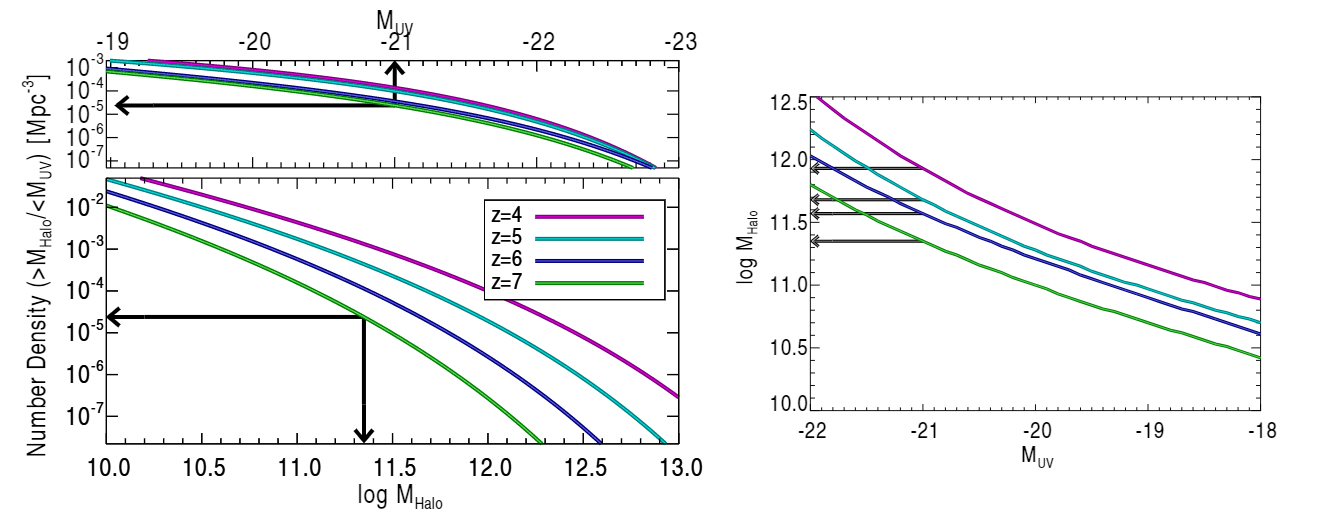
\includegraphics[scale=0.5]{Figuras/fink_1}
    \caption{\label{fig:fink1}Imagen sacada de \cite{finkelstein2015increasing}. Arriba a la izquierda: la función de luminosidad acumulada en z = 4, 5, 6 y 7. Abajo a la izquierda: funciones de masa acumulada del halo en z = 4, 5, 6 y 7, derivadas del promedio de volumen de las funciones de masa de snapshot de Bolshoi en los mismos rangos de redshift como los que definen las muestras de galaxias. Las flechas muestran los resultados de la coincidencia de la abundancia  en z = 7, donde las galaxias con $M_{UV} <-21$, que tienen $n(M_{UV} <-21) = 2.5 \times 10^{-5}Mpc^3$, tienen masas halo de registro $(M_h / M_\odot) = 11.35$. A la derecha: relación entre la magnitud absoluta de UV observada y la masa de halo derivada de la combinación de abundancia en los redshift de interés. Las flechas denotan las masas de halo en la magnitud de interés de $M_{UV} = - 21$.}
    
\end{figure}

Conociendo los datos de masa estelar de las galaxias con $M_{UV}<-21$ y la masa del halo de las que son huespedes dichas galaxias \cite{finkelstein2015increasing} enfrentan ambos datos en lo que denominan \textit{Stellar Baryon Fraction} (SBF) la cual la defininen como la fración $M_\star/M_h$ de masa estelar del halo versus la masa total (SMHM) en unidades de la fracción demateria bariónica cosmica $(\Omega_b/\Omega_m)=0.1669$. Comparando el SBF con el redsifht se encuentra que existe un aumento a medida que crece el redshift con un valor de $d SBF(z)/dz=0.024\pm 0.007$ como se muestra en la \textbf{Figura \ref{fig:finksbf}}.

\begin{figure}[h]
    \centering
    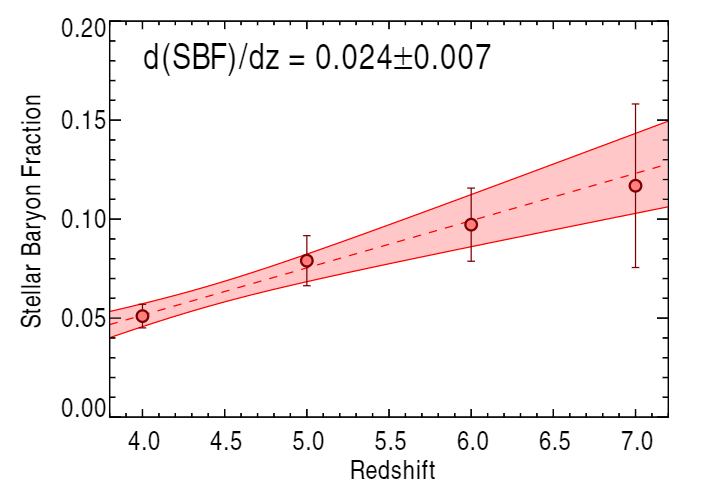
\includegraphics[scale=0.5]{Figuras/sbf}
    \caption{\label{fig:finksbf}Imagen sacada de \cite{finkelstein2015increasing}. La (SBF) en galaxias brillantes ($M_{UV} < -21$) de z = 4 a 7. Definimos SBF como la relación de masa estelar a halo en unidades de la fracción de masa de barión cósmica $\Omega_b / \Omega_m$. Encontramos que el SBF aumenta al aumentar el redshift, lo que puede ser responsable de la aparente falta de evolución en la magnitud característica $M^*_{UV}$ observada en este rango de redshift.}
    
\end{figure}


\begin{table}[h]
\begin{center}
\begin{tabular}{lcccc}
\hline \hline\\
Redshift & $\log n(M_{UV}<-21)$ & $\log M_h$ & Median & SBF \\
	& (Mpc$^{-3}$)& $(M_\odot)$ &	$M_\star/M_h$	&	\\
\hline\\
z=4 & -3.86 & $11.93_{-0.03}^{+0.03}$ & 0.009$\pm$0.001 & 0.051$\pm$0.006\\
z=5 & -4.01 & $11.68_{-0.03}^{+0.04}$ & 0.013$\pm$0.002 & 0.079$\pm$0.013\\
z=6 & -4.45 & $11.57_{-0.03}^{+0.06}$ & 0.016$\pm$0.003 & 0.097$\pm$0.019\\
z=7 & -4.62 & $11.35_{-0.06}^{+0.09}$ & 0.020$\pm$0.007 & 0.117$\pm$0.043\\
\hline
\end{tabular}
\caption{\label{tab:finkelstein2} Propiedades de los halos de materia oscura de las galaxias estudiadas, sacada de \cite{finkelstein2015increasing}}
\end{center}
\end{table}

Dado que la mediana de las magnitudes de las muestras seleccionadas se encontraban muy cerca del valor $M_{UV}^*=-21$ el estudio decidio volver a calcular la evolución del SBF para magnitudes $M_{UV}=-21\pm 0.25$, de esta manera se obtuvo que la SBF volvía a tener una evolución positiva según crecía el redshift $d SBF(z)/dz=0.0123\pm 0.0041$, una pendiente con un $3\sigma$ de significancia. Con ello concluyeron que el SBF aumentaba con redshift.\\

Los resultados son comparados con los de \cite{behroozi2013average}, \cite{barone2014measurement}, \cite{lee2006large} y \cite{overzier2006clustering}, donde los autores encuentran que sus predicciones de los valores $\log(M_h/M_\odot)$ y SMHM son ligeramente mayores que las estimadas por otros métodos para los diferentes rangos de redshift escogidos, pero dichas diferencías son muy pequeñas y explicables según los autores por el hecho de que los estudios anteriores trabajan con muestras más debiles de luminosidad $M_{UV}<-20, -19$. Dichas similitudes al tratarse de metodologías distintas parecen corraborar los resultados predichos. \\

Sin embargo dichas diferencias hacen plantearse en el artículo los efectos de la dispersión en UV, aplicando las correcciones sacadas de la relación entre luminosidad y masa estelar lo que hace corregir la luminosidad en 0.3 dex. Recalculando las estimaciones de masa de halo se obtiene los valores de masa característica de $log(M_h/M_\odot)=1.65, 11.44, 11.36$ y $11.13$ para los rangos de redshift centrados en $z=4,5,6$ y 7 respectivamente. Esto hace aplicar una corrección de 0.2 y 0.25 dex por debajo de las estimaciones de la masa del halo lo que se asemeja más a los resultados de \cite{behroozi2013average}, \cite{barone2014measurement}, \cite{lee2006large} y \cite{overzier2006clustering}. Dicha variación es muy parecida entre los diferentes rangos de redshift lo que hace permanecer igual los resultados de evolución de la SBF, sin embargo si para redshift superiores los efectos sería más significativos.\\

Una fuente de posibles \textit{bias} en la estimaciones del SMHM son las numerosas suposiciones que se requieren para poder estimar la masa estelar del halo, ¿podría alguna de ellas explicar que las masas estelares permanezcan casí idénticas entre $z=4-7$ mientras la masa del halo va decreciendo? Dichas fuentes pueden ser el \textit{slope} de la función de masa inicial (IMF) calculada por la función de Salpeter., donde dicho \textit{slope} se ha considerado en masas altas constante en el los distintos rangos de redshift \textcolor{red}{Dejando a un lado la pendiente escogida de la función IMF, el tipo de función de IMF no creo que tenga mucho que ver ya que para masas altas todas las funciones coinciden bastante.}. Otra fuente de bias es la parametrización de SFH, la cual es potencialmente más problemática, aunque los resultados recientes indican que, al menos en promedio, los SFR a escala de galaxias son funciones suaves del tiempo. Para intenar ver si existen posibles errores sistemáticos graves en los cálculos de la masa estelar se ha comparado  los SED de los distintos rangos de redshift enfrentando el flujo medido de cada una de las galaxias medidas versus la longitud de onda. Esta comparación se ha escalado vertivalmente al nivel del redshift z=6 para así compara su forma. Se ha comprobado una gran concordancia entre las formas de los SED (\textbf{Figura \ref{fig:sed_finkelstein}}) para los distintos rangos de redshift lo que ha hecho casi descartar los errores sistemáticos graves en la estimación de la masa estelar. \textcolor{red}{Dando por buena la suposición de que con SED comparables podemos descartar fuertes efectso de bias, en dicha comparación no da ningún dato más que el visual, no compara los distintos sed con test estadísticos (o por lo menos no da los resultados). Si comparamos estos resultados con un test estadístico quizás si encontremos que existe un bias que pueda afectar a la conclusión de que la masa estelar permanece constante lo que podría afectar al resultado de que el SBF crece según el redshift.}\\

\begin{figure}[t]
\begin{center}
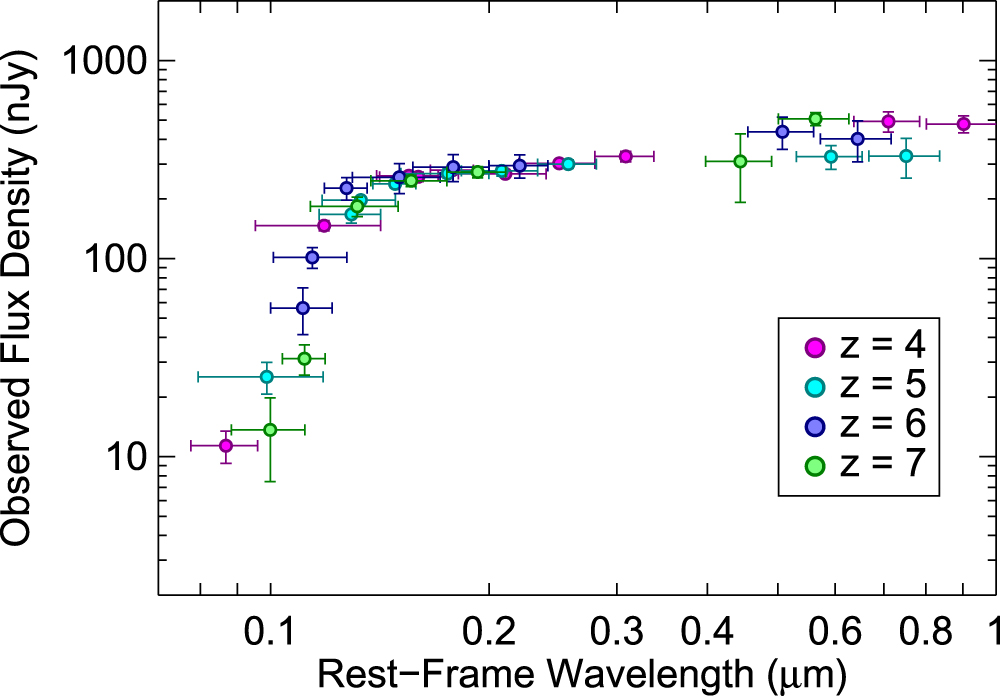
\includegraphics[scale=1]{Figuras/sed_finkelstein}
\caption{\label{fig:sed_finkelstein} Comparación del flujo y la longitud de onda de las distintas muestras de galaxias medidas en los diferentes rangos de redshift escalado verticalmente a $z=6$. Figura sacada de \cite{finkelstein2015increasing}.}
\end{center}
\end{figure}

Los efectos por la no detección de las galaxias polvorientas de formación estelar, es decir, las galaxias con un brillo muy alto en UV pero que son absorbido por su extremadamente alta cantidad en polvo (estas galaxias son denominadas galaxias sub-milimétricas) podrían sesgar nuestra masa de halo estimada (ya que estaríamos colocando nuestras galaxias observadas en los halos más masivos de nuestro volumen, que realmente estarían ocupadas por estas galaxias polvorientas) y además se verían intensificados junto con el hecho de que el número de densidad de estas galaxias puede variar con el redshift. Si la abundancia de SMG evoluciona con el redshift z>4, entonces no tener en cuenta estos sistemas sesgaría nuestras masas de halo de manera diferente en los diferentes redshift, sesgando nuestra evolución inferida del SBF. Los efectos de estas galaxias son descartados por \cite{finkelstein2015increasing}ya que considera que es altamente improbable una abundancia grande de este tipo de galaxias en redshift z=7 y que los efectos calculados en base a simulaciones de estas galaxias en redshift $z=4$ son del orden del $0.02$ dex en $log(M_h/M_\odot)$. Estas simulaciones se basan en el estudio de estas galaxias realizado en \cite{casey2014dusty} donde estiman la abundancia de este tipo de galaxias en $z\sim 2$ y dan una estimación de la evolución según el redshift. \textcolor{red}{La detección de ALMA de un gran número de galaxias masivas a $z>3$ en el campo CANDELS \citep{wang2019dominant} indetectables con el HST pone en cuestión este punto, ya que podría indicar una presencia relevante de este tipo de galaxias lo que modificaría los resultados expuestos en este paper.}\\

\subsubsection*{Discusiones}
\textcolor{red}{Revisar el paper de \cite{wang2019dominant} el cual ha detectado un cúmulo de galaxías muy masivas con bajo brillo UV debido al polvo a $z>3$ indetectables con HST y en el campo CANDELS, esto podría dar más info al trabajo.}\\

El artículo de \cite{finkelstein2015increasing} plantea dos posibilidades que entran en contradicción con los hechos observados y que con estas observaciones es imposible de dilucidar más a allá de las siguientes suposiciones.

\begin{enumerate}[I) ]
\item El primero de los escenarios posibles es que el gas galáctico a alto redshift tenga una mayor superficie de densidad $\Sigma_g \propto f_{gas}M_h^{1/3}(1+z)^2$ donde $f_{gas}$ denota la fracción de gas enfriado, es decir, en fase virializada. \textcolor{red}{No sé de donde sale dicha hipótesis y relación matemática, hay que revisar esta suposición en la bibliografía y sobre todo en \cite{krumholz2011universal}.} El tiempo típico de caída libre para cual para el cual el ratio de conversión de gas a estrellas es proporcional a él, aunque sea con una constante de proporcionalidad pequeña \citep{krumholz2011universal}, tiene la propiedad de que $t_{ff}\propto (1+z)^{-3/2}$. Sin embargo, las masas de los progenitores más masivos (MMP) de los halos que hospedan a nuestras galaxias observadas responden como $M_{h,MMP}(z')=M_h(z)e^{-\alpha(z'-z)}$ donde $\alpha \approx 1$ y $z'>z$ es el redshift del progenitor. Por lo tanto podemos calcular el tiempo $t_{grow}$ que tarda el progenitr en duplicar su masa.
$$t_{grow}\sim \left[(1+z)H(z)\frac{d}{dz}\ln M_{h,MMP}\right]\propto (1+z)^{-5/2}$$
Esto significa que el ratio entre el tiempo de caida libre y el tiempo el cual el halo duplica su masa es proporcional $t_{ff}/t_{grow}\propto (1+z)$, sugiriendo que si los progenitores más pequeños no son eficientes en su formación estelar no contribuyendo con una masa estelar sustancial a la rama principal, debería ser progresivamente más difícil en los redshift altos convertir el gas adquirido en nuevas estrellas. \textcolor{red}{Al ser mas dificil esa conversión en masa estelar del polvo acretado por las fusiones el ratio de masa estelar y masa halo ha de ser menor. Por ejemplo, si un halo menor se fusiona con un progenitor en la rama principal en redshift altos va a tener mucho menos tiempo para que formar estrellas mientras por lo que la masa estelar no se ve afectada y el ratio de SMHM no se modifica. Sin embargo, en redshift mas bajos va a tener mucho más tiempo para formar nuevas estrellas y por tanto producto de la fusión se van a poder formar nuevas estrellas que harán que aumente el SMHM con respecto al que había antes, esto debería de producir un aumento del SBF a medida que decrece el redshift contrario de lo que ocurre.}

\item En segundo lugar, la metalicidad del gas y la abundancia de polvo asociada parecen disminuir con el aumento del redshift y la disminución de la masa. Ya que el polvo y la metalicidad del gas son dos potentes herramientas en el enfriamiento del gas y en la obstaculación de la radiación UV, la tendencia observada del decrecimiento de la abundancia de polvo según aumenta el redshift podría tener un efecto dramáticoen la abundancia de gas frío ($T<1000 K$) para el cual parece que ocurre la formación estelar. La caida de la abundancia del gas frío a medida que crece el redhsift pordría indicar también un ratio de formación estelar menor. \textcolor{red}{El descubrimiento de \cite{wang2019dominant} de nuevas galaxias masivas fuera del alcance del HST podría echar a bajo esta suposición pues no se tiene en consideración la posible cantidad de polvo que pueden tener estas galaxias invisibles para el HST.}
\end{enumerate}

\textcolor{red}{En ambos escenarios la SFR es mucho más bajo en redshift altos lo que hace suponer que el SMHM es más bajo a medida que avanzamos en redshift, contrario a lo que se puede ver en el paper de \cite{finkelstein2015increasing}. Sin embargo, el trabajo de \cite{wang2019dominant} descubre galaxias con una gran formación de estelar en $z>3$, sin embargo no explica el porque parece que el SFR se mantuviera en dicho rango de redshift solo que es más alto de lo que se esperaría, ¿no?} \\

Todo esto sugiere una tendencia contraría a la observada donde el SBF descendiera a medida que se avanzaen redshift. Las especulaciones que realiza \cite{finkelstein2015increasing} para la explicación del aumento del SBF discuten diferentes especulaciones:
\begin{itemize}
\item Las observaciones implican unamenor cantidad de gas frío disponible para la formación de estrellas en redsift bajos lo cual se podría explicar por el descenso de la densidad en el universo a medida que decrece el redshift. La transición de la fase del gas de caliente a fría ocurre en densidades de $\sim 0.1-1$ cm$^{-3}$ lo que podría implicar una menor fracción de masa de gas neutral en fase fría en redshift bajos. \textcolor{blue}{Además, la naturaleza del colapso del gas en el disco depende mucho de si la estructura gaseosa central (normalmente en forma de discos nubosos) está autogravitando de manera violenta. La formación estelar es mas eficiente en grandes nubes de gas autogravitando donde divhas nubes se han observado formando estrellas en gran eficiencia en $z\sim 3$}.

\item Otra posibilidad es que estamos siendo testigos de los efectos del crecimiento del medio circumgaláctico (CGM) al rededor de las galaxias. Observaciones con el \textit{Cosmic Origins Spectrograph} en el HST a revelado halos de gas ionizado en bajos redshift que contenían una fracción significante de material bariónico sintetizado en metales. Es probable que el CGM creciera con el tiempo en forma del material empujado por las ondas de choque de ls supernovas más violentas incrementando la temperatura del gas. El gas reprocesado podría haberse depositado en un CGM caliente e ionizado y haber inhibido la conversión de la fase del gas a fría. Sin embargo, la física del CGM aún no se comprende muy bien.\\

\item Por último los \textit{feedback} que construyen el medio circumgaláctico podría ser menos eficiente en redshift más altos incrementando la cantidad de gas frío disponible en la formación estelar. Se podría esperar que los efectos de los \textit{feedback} fuesen menos efectivos en redshift altos ya que los halos son más densos y la masa tiene una mayor velocidad circular. Esto dificultaría expulsar el material de la galaxia al CGM o incluso al exterior del halo. Calculando las velocidad circulares sin embargo encuentran que decrecen a medida que crece el redshift lo que facilitaría la expulsión de material en redshift altos entrando en conflicto con lo observado. Sin embargo los efectos de los feedback también podrían evoluciona con el tiempo. Al decrecer la densidad la energía de lasexplosiones de supernova pueden transmitir una mayor cantidad de energía incrementando el tiempo de enfriamiento del gas circundante y por tanto inhibiendo la formación estelar. Otro mecanismo de \textit{feedback} son los AGN los cuales también pueden aumentar el tiempo d eenfriamiento reduciendo la SFR. Este tipo de \textit{feedback} requiere de un agujero negro supermasivo y aunque existen algunos ejemplos de AGNs a my altos redshift, la función de luminosidad de éstos parece decrecer rápidamente a partir de $z>3$, habiendo observado recientemente que la parte final de la función de luminosidad UV galáctica es más brusca que la función de masa de halo en $z=6$, pero no en $z=7$, lo que hipotéticamente podría explicarse si el \textit{feedback} en galaxias brillantes de los primeros AGNs volviera a partir de $z\leq 6$. Sin embargo, los detalles de como los AGNs interactúan con la galaxia y sus alrededores, particularmente en estas épocas, es muy incierto por lo que no es del todo claro si la acreción del agujero negor tiene algún efecto significativo en la evolución del crecimiento galáctico.
\end{itemize}

De todos estos escenarios \cite{finkelstein2015increasing} consideran más factble el último, donde los efectos de los \textit{feedback} decrecen con el redhift inhibiendo la formación estelar en redhisft más bajos.\\

A pesar de las especulaciones anteriores, la consecuencia de que incremente la disponibilidad de gas frío en redshift altos es intrigante. Los resultados en $z=6,7$ muestran que el $\sim 10-12$\% del complemento cósmico de bariones se ha transformado en estrellas. El resto de bariones han de permanecer en estado fase de gas siendo más abundante la fracción de gas en redshift altos que en bajos. Una alta fracción de gas en redsift altos no es esperable y será pronto confirmada por el ALMA \textcolor{red}{Ver si existe este resultado}.\\

Por último el paper de\cite{finkelstein2015increasing} analiza los posibles descendientes de las galaxias observadas concluyendo que los halos en redshift 2 han de tener masas similares a las que hospedan SMGs siendo este tipo de galaxias un candidato plausible a descendiende de las galaxiás brillantes UV observadas.

\subsubsection*{Conclusiones}

Recientes observaciones han mostrado que la luminosidad UV característica $M_{UV}^*$ no evoluciona significativamente entre los $z=4-7$, lo cual es inesperado dado el descenso general en la densidad de SFR cósmico junto con el crecimiento del redshift. Para investigar los efectos físicos detrás de las observaciones de la no evolución del $M_{UV}^*$ \cite{finkelstein2015increasing} ha inspeccionado a población estelar en galaxias brillantes UV en $z=4-7$ con los siguientes resultados.:
\begin{enumerate}[$\star$]
\item Galaxias con $M_{UV}^*<-21$ aparentan tener propiedades muy similares entre los $z=4-7$, incluyendo la masa estelar, la atenuación del polvo y el SFR.

\item Relacionando la función de luminosidad con la función de masa del halo de las simulaciones de Bolshoi se ha encontrado que las galaxias $M_{UV}<-21$, las cuales se han medido con un $\log M_\star/M_\odot=9.6-9.9$, viven en halos de $\log M_h/M_\odot=11.93-11.35$ entre los redshift 4 y 7 respectivamente. Por tanto la fracción estelar bariónica crece con una significancia de $3.2\sigma$ con el aumento del redshift.

\item La tendencia observada del SBF entra en contradicción con el crecimiento simple de las galaxias. Estas observaciones implican un cambio en las propiedades físicas  que gobiernan la formación estelar de $z>4$ las cuales, por ejemplo, reducirían la eficiencia de los \textit{feedback} de supernova a medida que aumenta el redshift.
\end{enumerate}

En futuros estudios esperan aumentar el volumen de la muestra estudiada además de extender el estudio a redshift 8 y 9. Por último se espera que con ALMA se pueda detectar la emisión de polvo que permita borrar los efectos de \textit{bias} producidos por él, sino que probar que la reserva de gas aumenta con el redshift probando que en redshit altos existiera una mayor cantidad de gas disponible para la formación de estrellas explicando el crecimiento del SBF con el redshift.\\

\textcolor{red}{
Algunas de las concluisiones y dudas generales que me he sacado de este artículo son:}
\begin{enumerate}[$\star$]
\item \textcolor{red}{Una de las primeras intrigas del artículo es el origen del trabajo, el cual intenta explicar por que la luminosidad característica de las funciones de luminosidad en los $z=4-7$ se mantiene constante. Se observa que aunque las galaxias en general tienden a decrecer en densidad mientras se aumenta redshift las galaxias brillantes permanecen constantes. Esto puede ser un efecto \textit{bias} provocadas quizás por las galaxias no observables comos las descubiertas con el ALMA \citep{wang2019dominant}, o si no fuera un sesgo observacional quizás es un indicador de que las galaxias brillantes se formaron primero.}

\textcolor{red}{
\item Por otro lado los margenes de error de las medidas de masa estelar, SFR y edad de las galaxias  parecen un poco amplios lo cual podría provocar confusiones en las conclusiones de que el SFR se mantiene constante donde se debería decir que no existe una dependencia significativa con el redshift con los margenes de error dados. He descargado los datos de las observaciones del paper para revisar dichos cálculos junto con las observaciones de Wang para así con RAMSES replicar los cálculos. Además la idea de asociar las galaxias según ranquin de masa halo y masa estelar no lo termino de entender muy bien.}

\textcolor{red}{
\item El principal efecto de \textit{bias} que puede haber influido en este trabajo es la detección de galaxias masivas no detecables en las observaciones. Estas galaxias podrían influir en la relación de masa estelar masa halo de una manera distinta en cada redshift si la densidad en número de éstas varía con el redshift trastocando los resultados por completo del SBF. Este efecto es descartado por el artículo ya que dichas observaciones no se conocián al ser muy posteriores.}
\end{enumerate}
\newpage
\bibliographystyle{plainnat}
\bibliography{references}

\end{document}